\setcounter{section}{-1}
\section{Motivation und Einführung}
\label{sec:para0}

\nextlecture
\subsection*{Kryptologie}
	Die \textbf{Kryptologie} besteht aus den folgenden beiden Gebieten: \marginnote{[1]} 
	\begin{description}
		\item[Kryptographie:] Studium mathematischer Techniken zur Verschlüsselung von Informationen oder geheimen Nachrichten und dem Schutz von Daten.
		\item[Kryptoanalyse:] Beschreibung der Rückgewinnung von Informationen aus verschlüsselten Texten, der Entschlüsselung.
	\end{description}
Oft meint man mit "Kryptographie" die Kryptologie. \\

Früher wurde die Kryptographie vor allem im militärischen oder diplomatischen Sektor verwendet, heutzutage steht in unserer vernetzten Welt vor allem auch der praktische Nutzen im Alltag im Vordergrund: im Internet einkaufen, Online-Banking, persönliche Daten geheimhalten bzw. Datenschutz, Nachrichten und Dokumente digital unterschreiben etc. Das Internet liefert schnelle Informationswege über öffentliche Kanäle, die leicht abgehört werden können, sodass die Verschlüsselung schützenswerter Daten unumgänglich wird. Auch die Möglichkeit zur Signierung wird nötig, weil sehr leicht Absenderangaben gefälscht werden können. Eventuell nicht abhörsichere Kanäle können außer dem Internet aber auch Briefe, Radio, Boten, etc. sein. \\

Bei der \textbf{symmetrischen Verschlüsselung} von Daten gibt es einen Sender $S$ und einen Empfänger $E$, die sich beide auf einen gemeinsamen Schlüssel geeinigt haben, der zum Ver- und Entschlüsseln dient. Beim \Index{Caesar-Code} z.B. ist dies die Vereinbarung, jeden Buchstaben durch den dritten nachfolgenden im Alphabet zu ersetzen, also $A \mapsto D, B \mapsto E, C \mapsto F$, usw. Die Entschlüsselung ist klar. Derartige \textbf{monoalphabetische Chiffrierungen}, bei der jeder Buchstabe des Alphabets stets durch denselben Geheimtextbuchstaben chiffriert wird, sind durch Häufigkeitsanalysen durch einen Angreifer, der die verschlüsselten Nachrichten abhört, sehr leicht zu entschlüsseln. Übrigens gibt es auch heutzutage PDF-Verschlüsselungsprogramme, die so arbeiten! 

In dieser Vorlesung behandeln wir die heutzutage gängigen modernen Methoden, die als sicher gelten. Worauf diese starke Sicherheit beruht, hat mathematische Gründe, die wir besprechen möchten. Vor allem interessiert uns, wie und welche Mathematik in die Kryptologie kommt, sodass wir deren Verfahren verstehen können. \\

Die Anwendungen erfordern die Lösung folgender Probleme bei symmetrischen Verschlüsselungsverfahren:
\begin{itemize}
	\item Schlüsselaustausch über öffentliche Kanäle (\textbf{öffentliche Schlüssel})
	\item Verschlüsselung ohne vorherigen Schlüsselaustausch (mit \textbf{geheimen Schlüsseln}, die nicht versendet werden)
	\item Digitale Signierung und Autentifizierung
\end{itemize}
Dies können \textbf{asymmetrische Verfahren} leisten (auch \textbf{Public Key-Kryptographie} genannt) und gehen zurück auf Ideen von Diffie\footnote{Whitfield Diffie, \url{http://de.wikipedia.org/wiki/Whitfield_Diffie}} und Hellman\footnote{Martin Hellman, \url{http://de.wikipedia.org/wiki/Martin_Hellman}} aus den 70er Jahren: \\

Jeder Nutzer eines Kommunikationskanals hat einen privaten Schlüssel, den er geheim hält und niemand sonst kennt, sowie einen öffentlichen Schlüssel, den jeder einsehen kann. Eine Nachricht wird dann unter Ausnutzung einer Funktion $x \mapsto f(x)$ verschlüsselt, die zwar leicht zu berechnen, aber praktisch nur mit Kenntnis des privaten Schlüssels des rechtmäßigen Empfängers entschlüsselt werden kann. Der Sender der Nachricht wird dafür den öffentlichen Schlüssel des Empfängers zur Verschlüsselung benutzen. Eine derartige Funktion heißt \Index{Einwegfunktion}.

\minisec{Beispiele}
\begin{itemize}
	\item \Index{RSA-Verfahren}: $(p,q) \mapsto p \cdot q$ mit $p,q$ prim.
	\item \Index{ECC-Verfahren}: $x \mapsto mx$ in einer Gruppe auf einer elliptischen Kurve.
\end{itemize}

In einem ersten Teil der Vorlesung stellen wir gängige Verfahren dar, die leicht mit dem Zahlring $\ZZ$ und Strukturen darin realisiert werden können. Dabei werden wir nur einige Hilfsmittel der elementaren Zahlentheorie entwickeln und dafür heranziehen. In einem zweiten Teil studieren wir die Eigenschaften elliptischer Kurven als interessante geometrische und arithmetische Objekte, die sich in der Praxis der Kryptographie als nützlich erwiesen haben. Wir besprechen dann auch die Sicherheit und Implementierung dieser Verfahren und vergleichen sie miteinander.

\subsection*{Elliptische Kurven}
Was sind elliptische Kurven? Jedenfalls sind elliptische Kurven \textbf{keine} Ellipsen. Ellipsen lassen sich durch Gleichungen der Form
\[ \enbrace*{\frac{x}{a}}^2 + \enbrace*{\frac{y}{b}}^2 = 1 \text{ mit } a,b \in \RR \setminus \setnull \]
beschreiben. Durch die Parametrisierung $x(t) = a \cdot \cos(t), y(t) = b \cdot \sin(t)$ ergibt sich für die Bogenlänge der Ellipse ein elliptisches Integral zweiter Art, nämlich
\[ \int_{0}^{2\pi} \sqrt{ \enbrace*{\frac{dx(t)}{dt}}^2 + \enbrace*{\frac{dy(t)}{dt}}^2 } dt = 4 \int_{0}^{2\pi} \sqrt{ a^2 \cos^2(t) + b^2 \cdot \sin^2 (t)} dt \]
Im Allgemeinen lässt sich dies nicht elementar integrieren (außer natürlich, falls $a = b$, d.h. ein Kreis vorliegt). Mit Hilfe von elliptischen Kurven findet man jedoch nicht-elementare Stammfunktionen für diese Integrale ($\Rightarrow$ Funktionentheorie). Aufgrund dieses Zusammenhangs haben elliptische Kurven ihren Namen, sie haben ansonsten nichts mit Ellipsen zutun. \\

Was sind nun elliptische Kurven? Es sind "abelsche Varietäten der Dimension 1". Elliptische Kurven sind spezielle algebraische Kurven über einem Körper $k$. Es handelt sich dabei um glatte kubische Kurven, deren definierende algebraische Gleichung sich meist in die Form
\[ E \colon y^2 = x^3 + ax + b \text{ mit } a,b \in k \]
bringen lässt. Als Punktmenge haben wir dafür
\[ E(k) := \{ (x,y) \in k^2 : y^2 = x^3 + ax + b\} \cup \{ \oh \}, \]
die Kurve hängt nur von $a,b$ ab. Die Rolle des zusätzlichen so genannten "unendlich fernen Punkts" $\oh$ werden wir dabei noch näher beleuchten. \\

Zwei typische Beispiele für elliptische Kurven:
\begin{enumerate}[1)]
	\item $E_1\colon y^2 = x^3 + 17$, hier liegen sogar Punkte mit ganzzahligen Koordinaten auf $E_1$, nämlich $(-2,3), (-1,4), (2,5)$. Die Kurve besteht aus einer Zusammenhangskomponente.
	\item $E_2 \colon y^2 = x^3 + ax + b$, wenn $f(x) = x^3 + ax + b$ drei verschiedene Nullstellen hat, z.B. $a = -3, b= -1$. Die Kurve besteht dann aus zwei Zusammenhangskomponenten.
\end{enumerate}

\begin{figure}[h!]
	\centering
	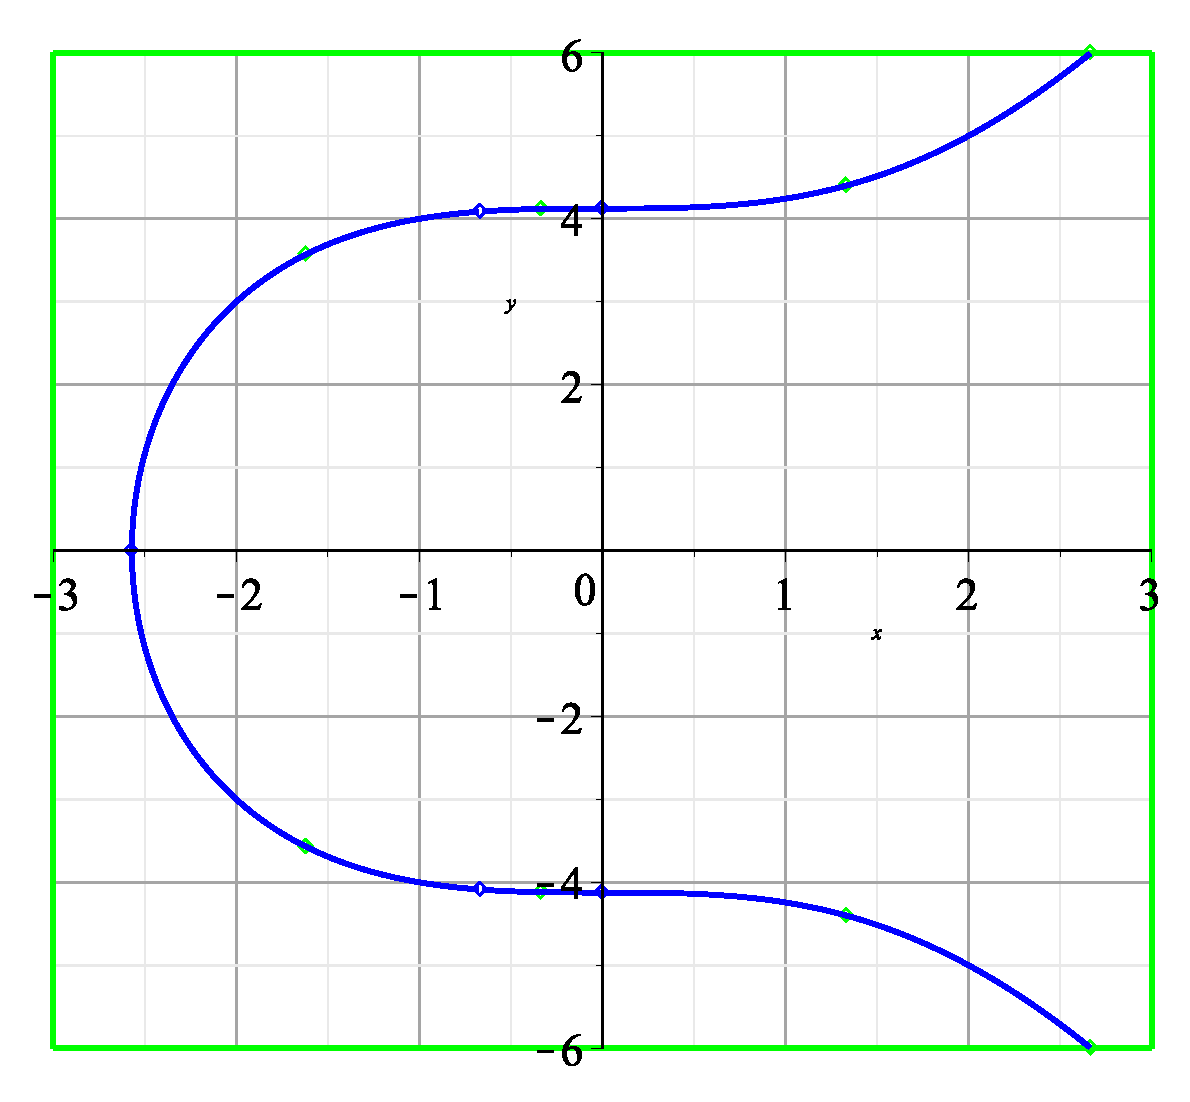
\includegraphics[scale=.3]{img/curve_0_1.eps} \hspace{2cm}
	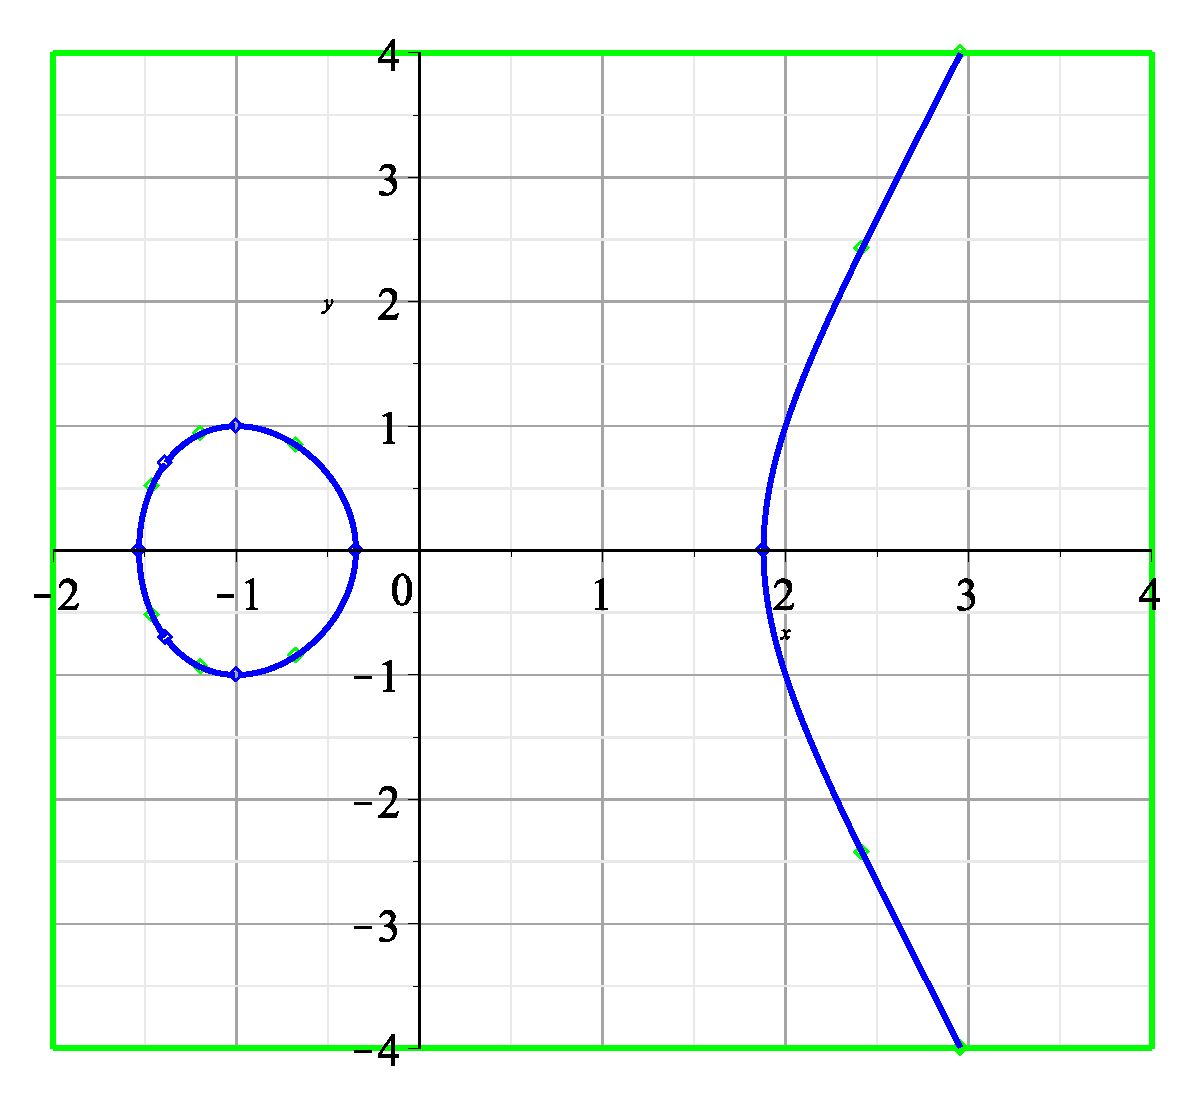
\includegraphics[scale=.3]{img/curve_0_2.eps}
	\caption{Die Kurven $E_1$ (links) und $E_2$ (rechts).}
\end{figure}
%\begin{figure}[h]
%	\centering
%	\begin{tikzpicture}
%	\begin{axis}[
%		scale only axis,
%		xlabel=$x$,
%		ylabel=$y$,
%		grid=major,
%		axis lines=middle,
%		inner axis line style={=>},
%		ymin = -5,
%		ymax = 5,
%		xmin = -3,
%		xmax = 3,
%		xtick={-3,-2,...,3},
%		ytick={-5,-4,...,5}
%	]
%	\addplot[color=red, thick, domain=-2.57128:3, samples=100] {(x^3+17)^(1/2)};
%	\addplot[color=red, thick, domain=-2.57128:3, samples=100] {-(x^3+17)^(1/2)};
%	\end{axis}
%	\end{tikzpicture} \hspace{2cm}
%	\begin{tikzpicture}
%	\begin{axis}[
%		scale only axis,
%		xlabel=$x$,
%		ylabel=$y$,
%		grid=major,
%		axis lines=middle,
%		inner axis line style={=>},
%		ymin = -5,
%		ymax = 5,
%		xmin = -3,
%		xmax = 3,
%		xtick={-3,-2,...,3},
%		ytick={-5,-4,...,5}
%	]
%	\addplot[color=red, thick, domain=-1.53208888:-0.347296, samples=100,unbounded coords=jump] {(x^3-3*x-1)^(1/2)};
%	\end{axis}
%	\end{tikzpicture}
%\end{figure}

\minisec{Bemerkung}
	Die kubischen Kurven $C_1\colon y^2 = x^3 - 3x +2$ und $C_2\colon y^2 = x^3$ z. B. sind jedoch keine elliptischen Kurven, weil diese nicht glatt sind. \\

\begin{figure}[H]
	\centering
	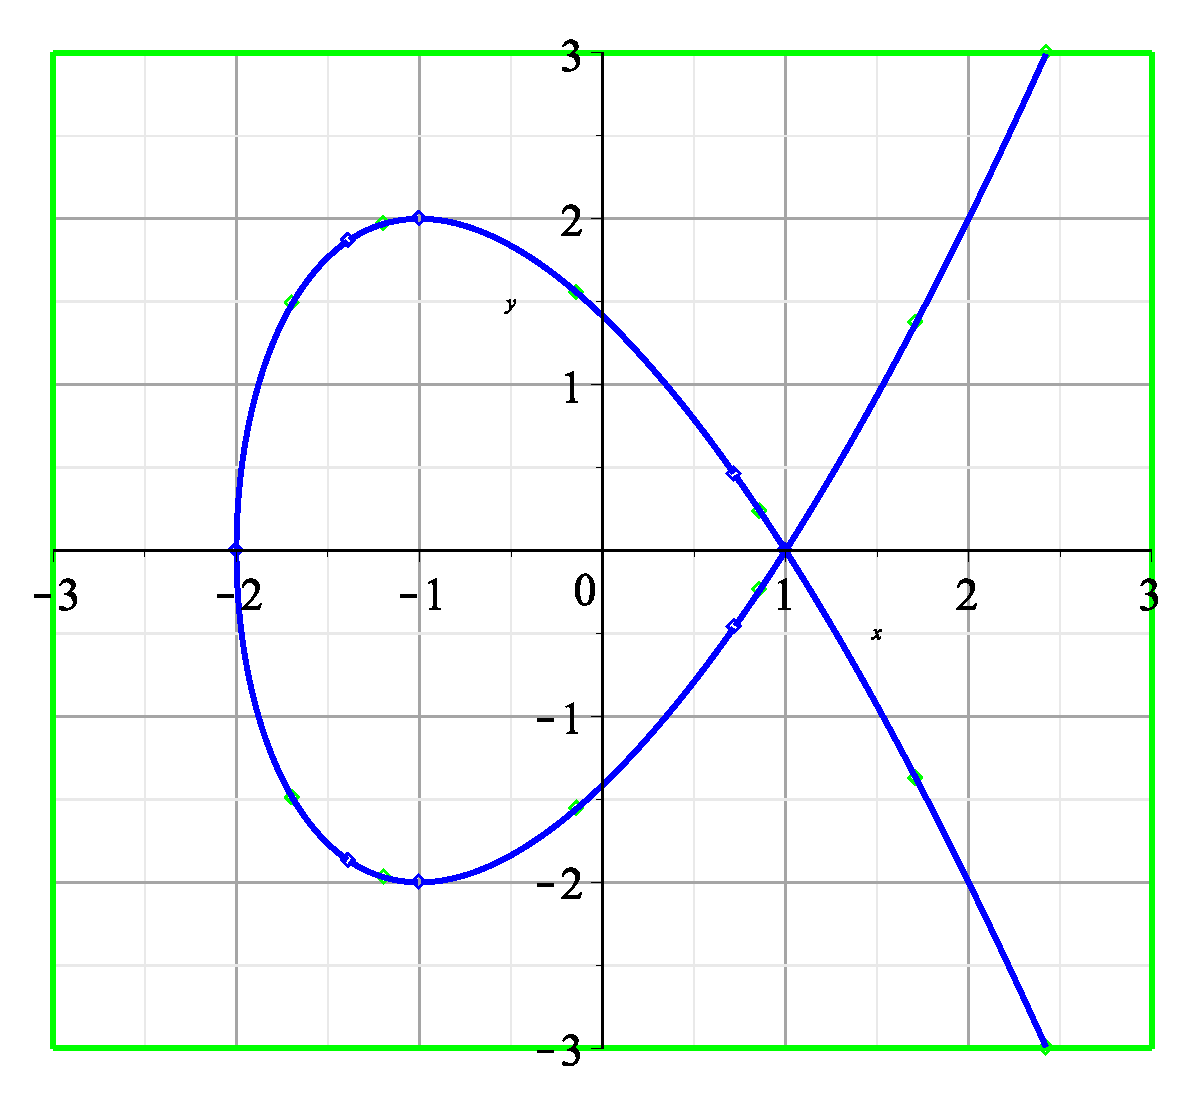
\includegraphics[scale=.3]{img/curve_0_3.eps} \hspace{2cm}
	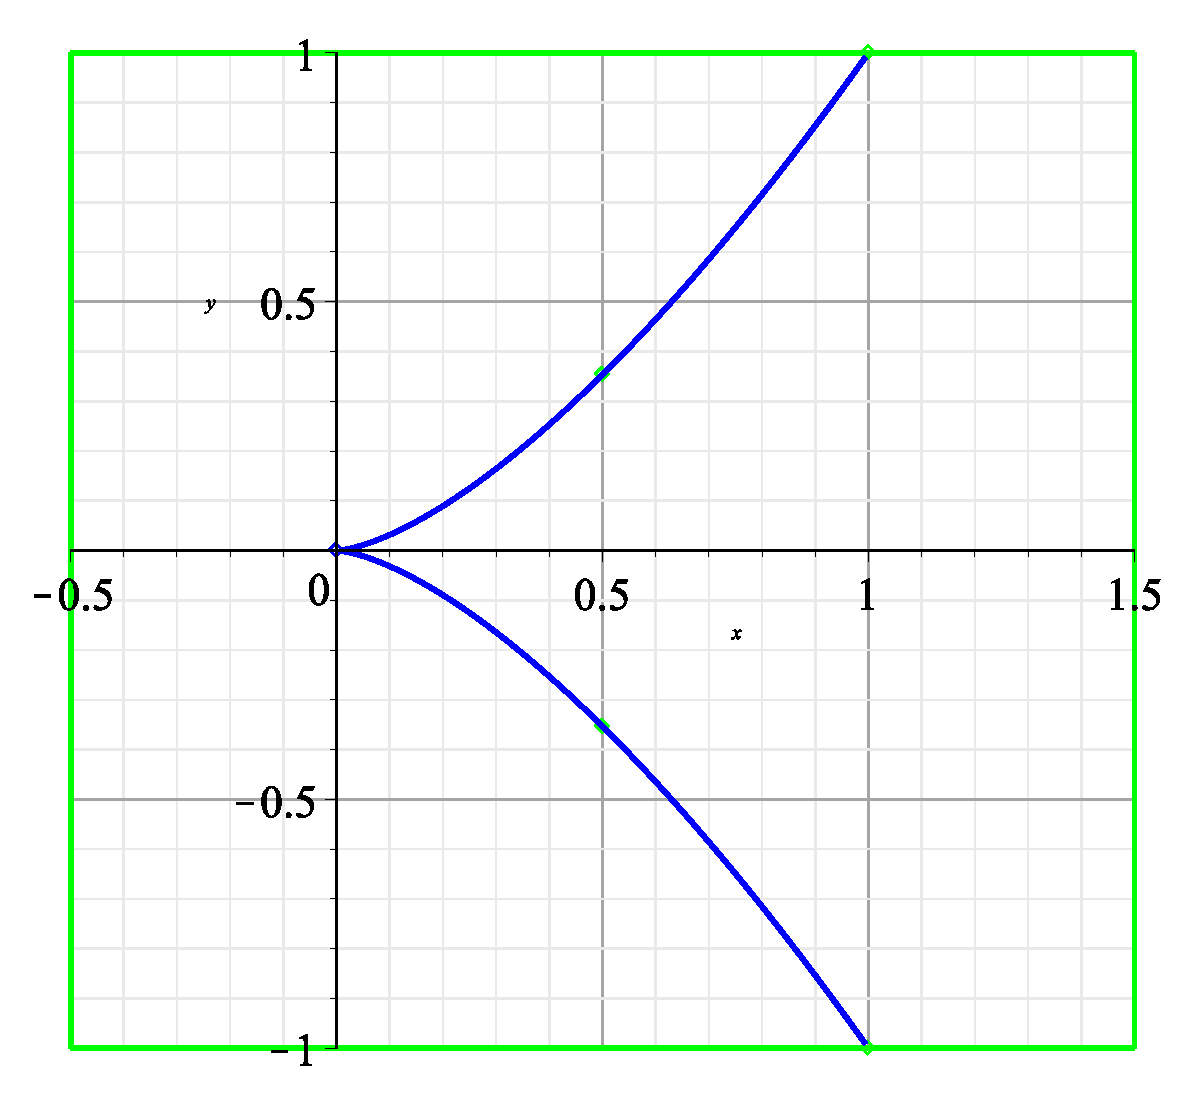
\includegraphics[scale=.3]{img/curve_0_4.eps}
	\caption{Die Kurven $C_1$ (links) und $C_2$ (rechts). $C_1$ ist nicht glatt im Punkt $(1,1)$, $C_2$ nicht im Punkt $(0,0)$.}
	\label{fig:bsp}
\end{figure}

Für die Kryptographie sind elliptische Kurven interessant, weil sich eine Verknüpfung auf ihrer Punktemenge definieren lässt, mit der diese zu einer Gruppe wird. Dabei gerade auch endliche Körper $k$ zuzulassen, macht diese Verknüpfung auf Rechenmaschinen realisierbar. Die Sicherheit der darauf beruhenden elliptic curve cryptography (ECC) beruht darauf, dass das Problem des diskreten Logarithmus auf einer elliptischen Kurve $E$, nämlich die Umkehrung der Funktion $P \mapsto mP$ für $m \in \NN$ fest, nach heutigem Wissensstand rechnerisch im Allgemeinen extrem schwer realisierbar ist.
\newpage